\documentclass[11pt]{article}
\usepackage[top=1.00in, bottom=1.0in, left=1in, right=1in]{geometry}
\renewcommand{\baselinestretch}{1.1}
\usepackage{graphicx}
\usepackage{natbib}
\usepackage{amsmath}
\usepackage{parskip}
\usepackage{wrapfig}

\def\labelitemi{--}
\parindent=0pt

\begin{document}
\renewcommand{\refname}{\CHead{}}

% \setlength{\parindent}{0cm}
% \setlength{\parskip}{5pt}

\title{Mapping trees with a Vertex} 
\author{Lizzie, with field help from Valentina Vitali}
\date{\today}
\maketitle
\begin{wrapfigure}{r}{0.5\textwidth}
\centering
    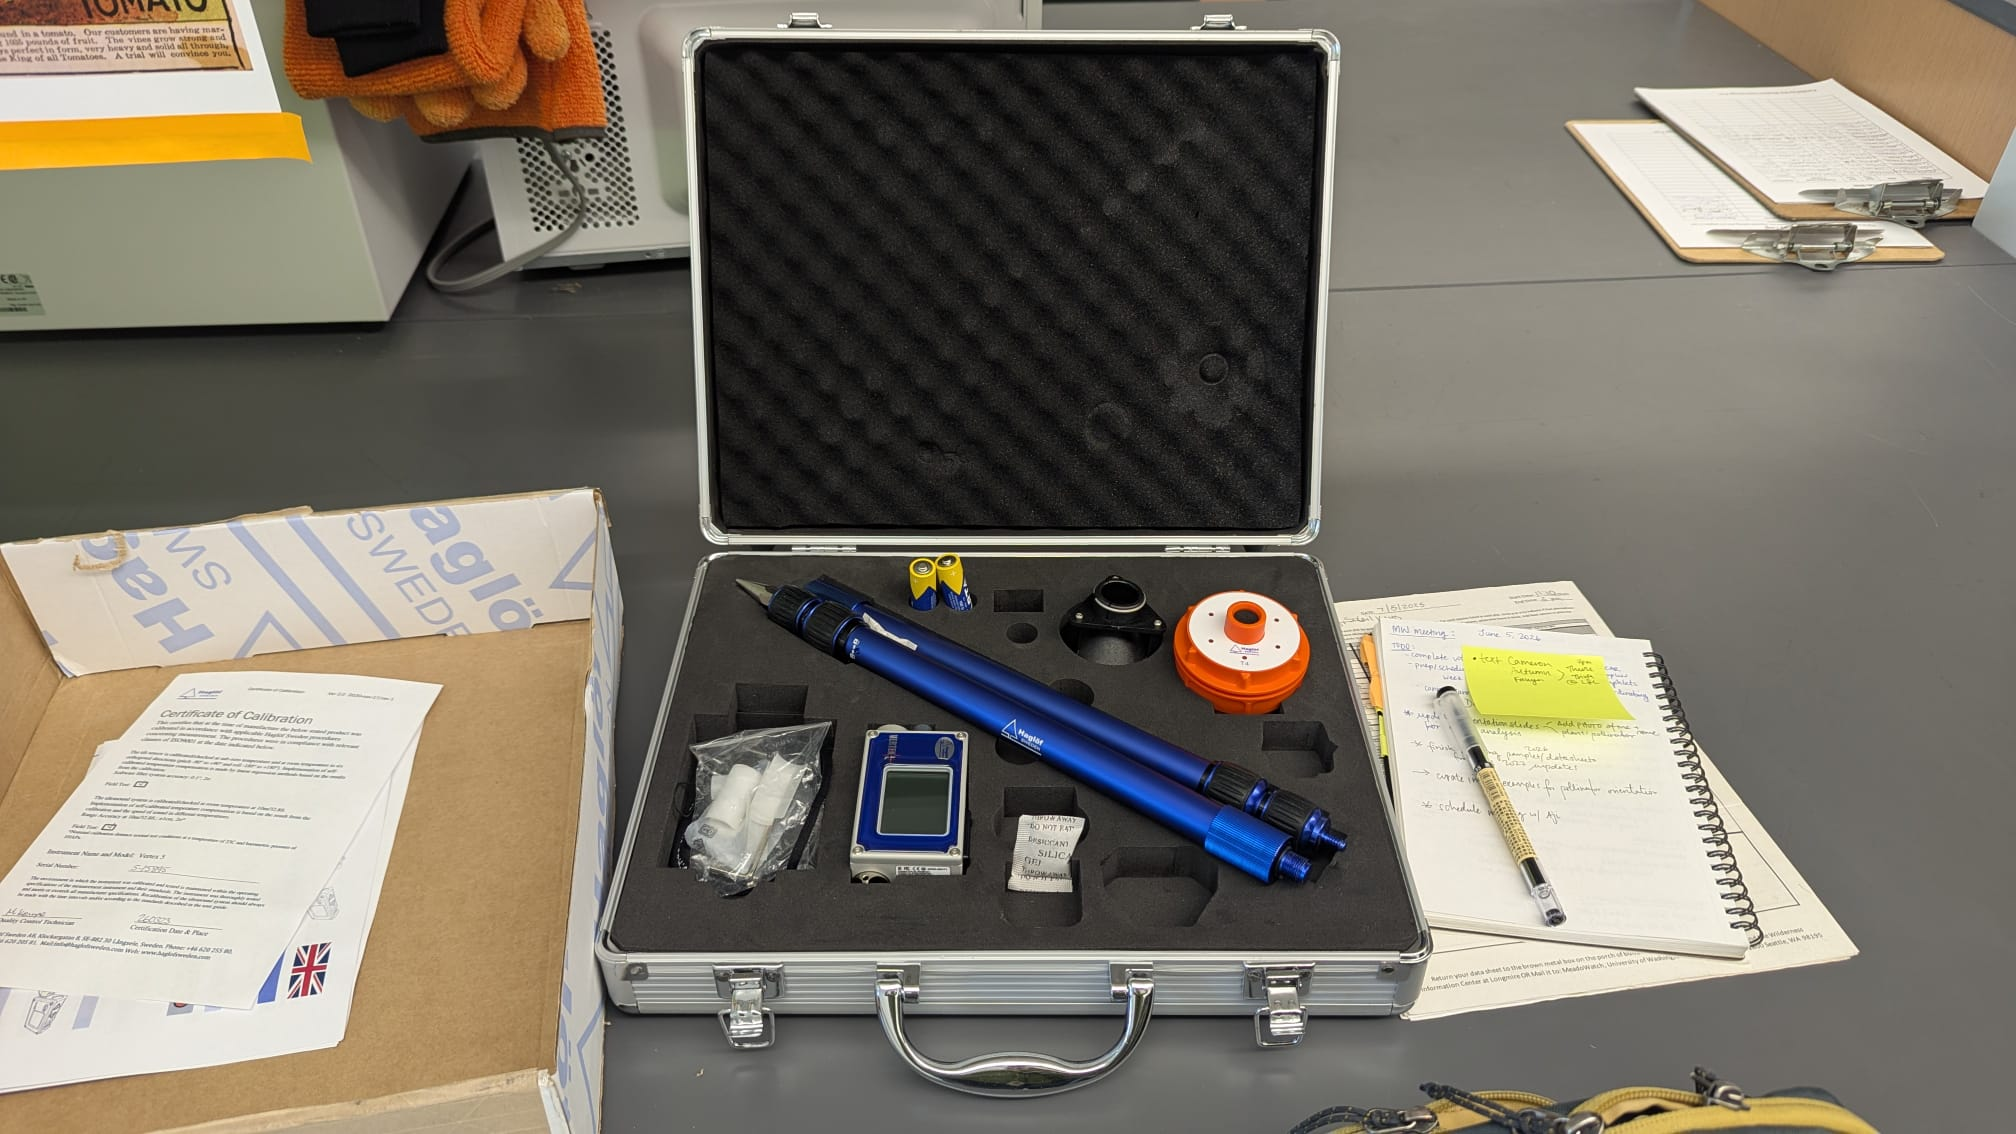
\includegraphics[width=0.48\textwidth]{images/WhatsAppVertex.jpg}
        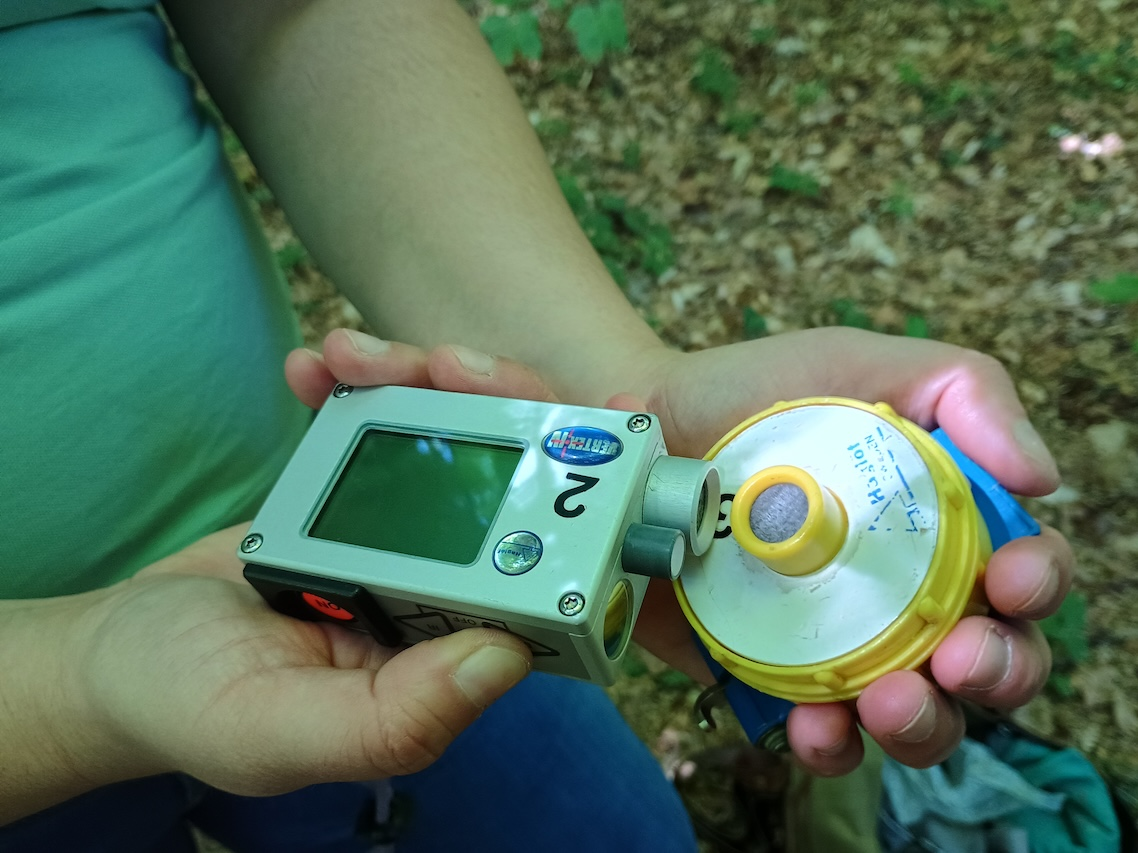
\includegraphics[width=0.48\textwidth]{images/Vertex2parts.jpg}
  \caption{The Vertex the lab bought (top). Slightly different model from the one Valentina has (below), but highly similar I suspect. Both have two parts: Transponder (yellow or orange) and Vertex (silver with a little screen). Be sure to review instructions on how to use it carefully and test it out before you head into the field}
  \label{fig:ourvert}
\end{wrapfigure}
\clear

\emph{Overview:} The Vertex is a two-part survey system (Fig. \ref{fig:ourvert}) that can help measure a suite of distances especially helpful for measuring trees to estimate neighborhood density and stand mapping. Be sure to try it out in advance as it makes quiet beeps and other things you need to notice and have down pat. For our purposes, it is measures the distance between the Vertex (rectangular device, Fig. \ref{fig:verttran}) and its transponder (circular, Fig. \ref{fig:verttran}) and tree height, which I describe below. (For MORA, I think we aim to match PSP sampling and so do not necessarily need tree height.) 

These are notes by Lizzie from learning how to use a Vertex (VI) with Valentina Vitali on 8 May 2026 in Zurich. We can use them to make a separate document on how to sample. 

\section*{Steps}



\clearpage
% \begin{minipage}[t]{0.55\textwidth} % Allocates 55% width to the list
\begin{enumerate}
\item Attach the transponder at breast height (roughly 1.3 m; similar to DBH) to a focal tree. You'll likely want to then GPS this tree, note it on your datasheet and measure its DBH. The steps below suggest how to measure a neighborhood of trees around a focal tree. 
\item If you want to take height of your focal tree, then walk away from the focal tree and use the height measuring setting to capture height. Vertex will prompt you to take multiple measurements and will also correct for slope etc. (though check if you need to set this up in settings or such, worries Lizzie). 
\item For neighborhood, it is best if one person stays with the clipboard (datasheet, Fig. \ref{fig:clipboard}) and focal tree and the other person runs around with the Vertex visiting each tree (when gathering the distance information with the Vertex, stay close to the tree you are measuring so the measurement is accurate). Ideally the person with the focal tree calls out which tree to go to, then writes down data from the person with the Vertex. 
\item Set a distance for the neighborhood (15 m? Depends on the trees and forests, 10 or 12 m can also work) and record all trees (possibly above some minimum DBH) around the focal tree. At each tree, be sure to collect (aall these out to the person recording data.):
\begin{enumerate}
\item Angle from focal tree
\item DBH 
\item Species
\item Distance from focal tree using Vertex distance measuring setting.  
\end{enumerate}
\item Mark each tree measured (with chalk for example). 
\item When all the trees around one focal tree are measured, take the transponder off the tree, go to next focal tree and repeat.
\item At the end of the work, take the batteries out of the Vertex and put it safely away. 
\end{enumerate}
% \end{minipage}

\section*{Helpful hints}
\begin{enumerate}
\item To keep best track of things and make it easier to write, the person at the focal tree may want to have the clipboard pressed flat between them and the tree (Fig. \ref{fig:clipboard}) and then methodically calls out to trees for the person with the Vertex to report on and measure. 
\item As the steps above suggest how to measure a neighborhood around a focal tree, to map a stand, you'll need to figure out overlapping circles or some other methods to capture all trees (then re-create the stand from those data; I don't believe Valentina does this so we'd need to figure out how to do it ourselves). 
\item You can do this faster with an additional transponder mounted on a pole, but be careful to make sure you capture the right transponder then!
\item Valentina does this when coring trees. Best with three people: one person coring, two people on mapping with Vertex. I have a few notes in my orange notebook on how to organize this best if we ever need it, 
\end{enumerate}

\section*{Equipment list (incomplete)}
\begin{enumerate}
\item Vertex system -- Valentina kept hers in a cute little tupper (when not in use take the batteries out)
\item Extra batteries
\item Clipboard with pencil attached via string
\item Compass 
\item Chalk (to make trees done) or maybe Forester's tape (I have no idea what that is, but Valentina mentioned it)
\end{enumerate}

\section*{Datasheets}
\emph{All should have a spot for date, site and who is collecting data.}
\begin{enumerate}
\item Focal tree information -- species, size, GPS, maybe time you started recording it 
\item Neighborhood -- focal tree, compass direction, distance, size, species ... what else? Maybe something about health or canopy or both?
\item Valentina has heard that noisy areas can be problematic for the Vertex (like standing right next to a gushing stream perhaps). 
\end{enumerate}

\clearpage

\begin{wrapfigure}{r}{0.5\textwidth}
\centering
    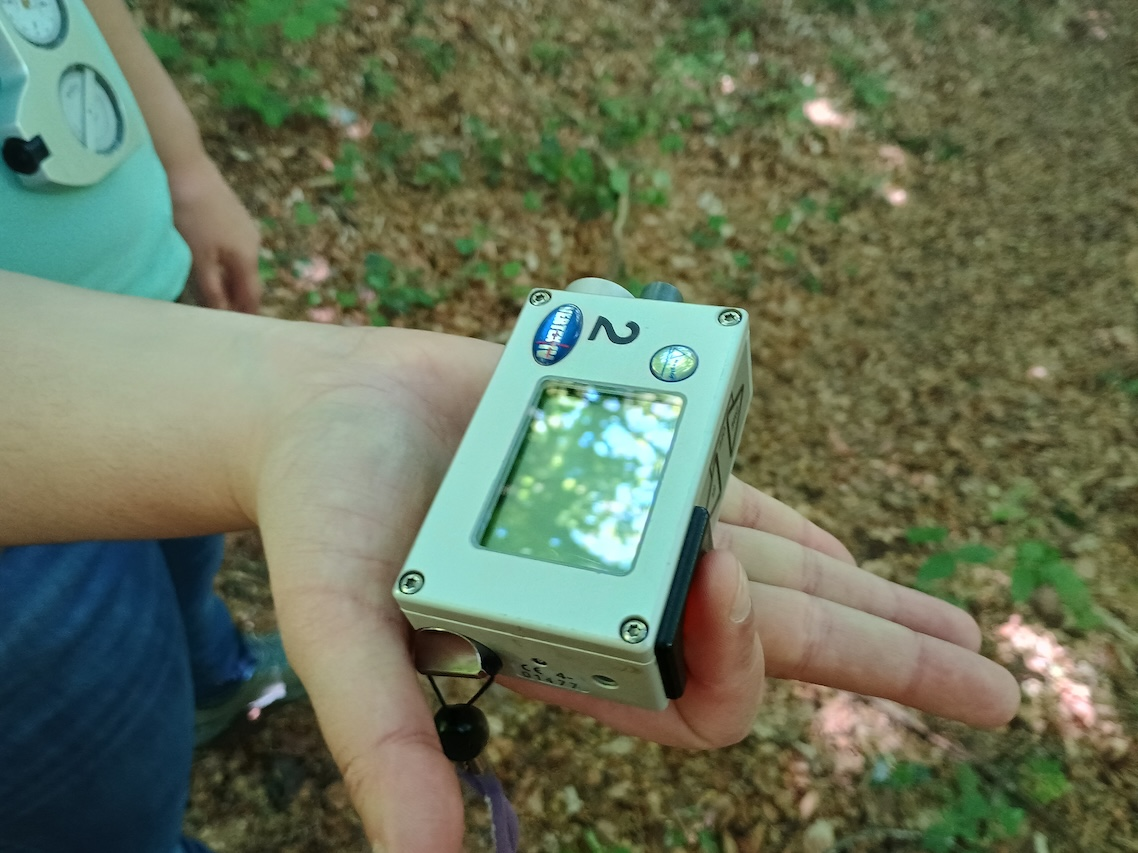
\includegraphics[width=0.48\textwidth]{images/Vertex.jpg}
    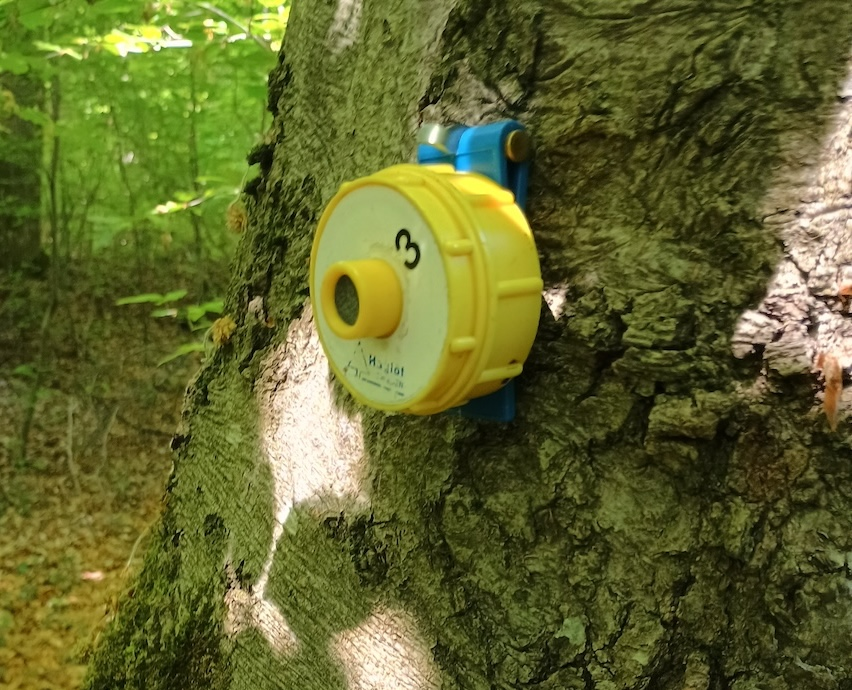
\includegraphics[width=0.48\textwidth]{images/VertexTransponder.jpg}
  \caption{The Vertex (top) and the transponder on a tree (bottom) waiting to communicate with the Vertex.} 
  \label{fig:verttran}
\end{wrapfigure}

\begin{wrapfigure}{l}{0.5\textwidth}
  \begin{center}
    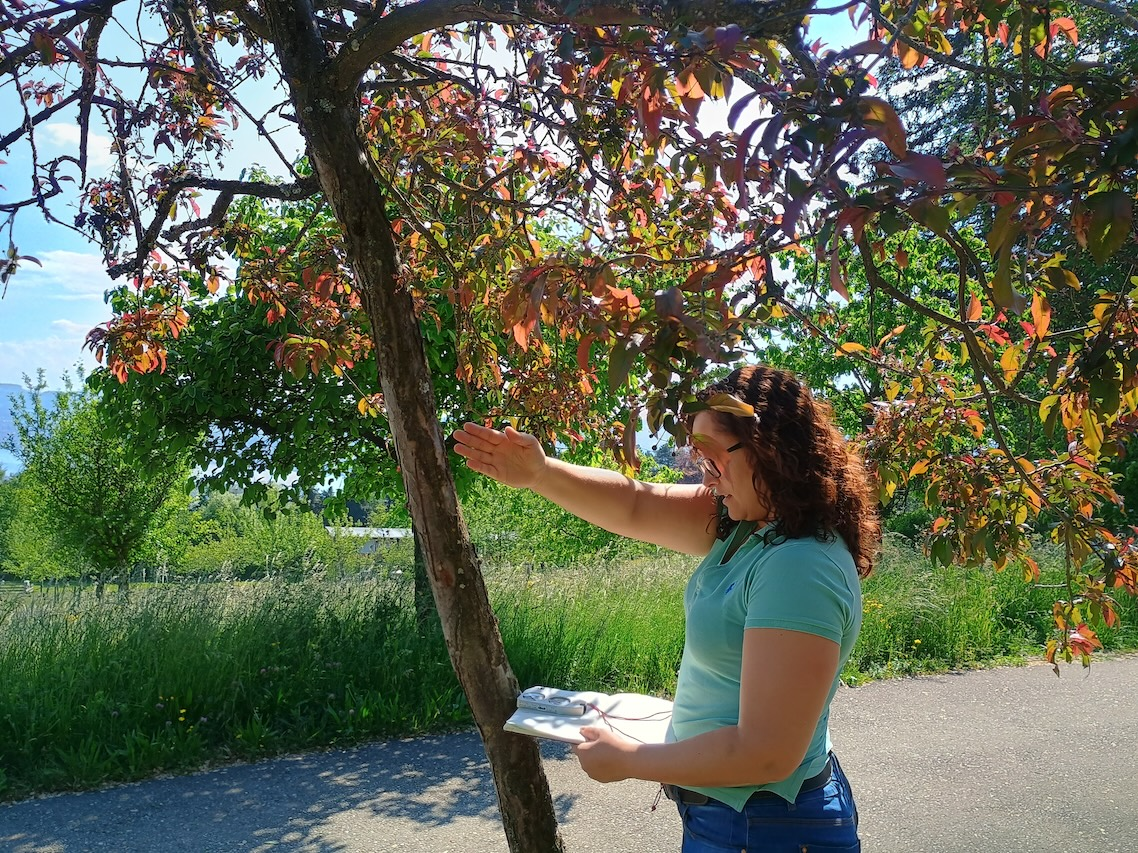
\includegraphics[width=0.48\textwidth]{images/ValentinaDemoClipboard.jpg}
  \end{center}
  \caption{Valentina showing how to hold the clipboard steady and call out trees for the person with the Vertex to measure.}
  \label{fig:clipboard}
\end{wrapfigure}

\begin{wrapfigure}{r}{0.5\textwidth}
  \begin{center}
    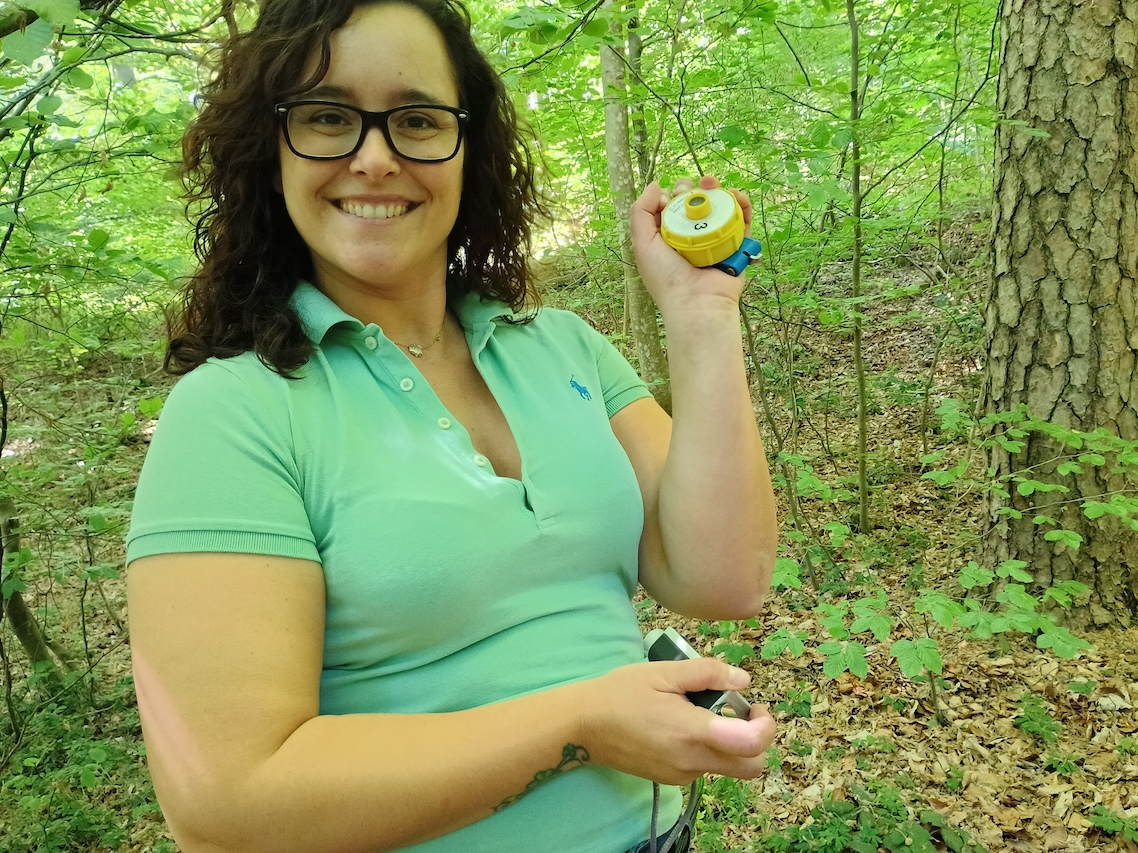
\includegraphics[width=0.48\textwidth]{images/ValentinaDemo.jpg}
  \end{center}
  \caption{Valentina Vitali showing the transponder and the Vertex is in her other hand. }
  \label{fig:valentina}
\end{wrapfigure}




\end{document}
